\documentclass[11pt]{article}
\usepackage[margin=1in]{geometry}
\usepackage{amsmath,amssymb}
\usepackage{graphicx}
\usepackage{booktabs}
\usepackage{xcolor}
\usepackage[colorlinks=true,linkcolor=blue,citecolor=blue,urlcolor=blue]{hyperref}
\usepackage{mdframed}

\newcommand{\Neff}{N_{\mathrm{eff}}}
\newcommand{\Sown}{S_{\mathrm{own}}}
\newcommand{\Sopp}{S_{\mathrm{opp}}}

\title{\textbf{A self-organising Thucydides trap --- v2}\\[2pt]
\large dynamic growth, deliberation by rollout, and war-driven alliances}
\author{M.\ Heltberg}
\date{Note, June 2026}

\begin{document}
\maketitle

\noindent\emph{Self-contained. Supersedes the v1 model (see
\texttt{NOTE\_selforg.tex} for the earlier lattice-free version and its
motivation). Code: \texttt{thucydides\_selforg\_v2.py}; figures
\texttt{make\_figures\_v2.py}; depth sweep \texttt{experiments\_v2.py}.}

\bigskip
\noindent This version was built around four design decisions and one new
mechanism that the v1 model lacked:
\begin{itemize}\itemsep1pt
\item growth rates that \emph{vary in time} (so any state can rise, not only the
  large ones);
\item no per-state capacity parameter;
\item prediction by explicit \emph{Monte-Carlo rollout} of future wars;
\item \textbf{war-driven absorption}: the defeated side is swallowed into the
  victor's alliance --- which is the concrete reason allies fight (to avoid
  losing their partners to the enemy bloc).
\end{itemize}
The Q\&A in \S\ref{sec:qa} answers four specific questions; \S\ref{sec:war}
gives the war rules in full and \S\ref{sec:example} a fully worked numerical
example.

% ====================================================================
\section{State and time}

$N=100$ states. State $i$ carries
\begin{center}
\begin{tabular}{ll}
$S_i\ge0$ & strength \\
$\gamma_i(t)$ & instantaneous growth rate (a slow stochastic process, below) \\
$x_i\in[0,1)$ & position on a 1-D ring (geography/ideology) \\
$n_i$ & deliberation depth (number of rollouts it can run) \\
$b(i)$ & alliance label; an \emph{alliance} (bloc) is the set $\{j:b(j)=b(i)\}$ \\
$\widehat{\dot S}_i$ & its online estimate of its own growth slope \\
\end{tabular}
\end{center}
Time advances in \emph{rounds} of length $\Delta=n_{\rm sub}\,dt=1$. Each round:
(1) integrate the growth SDE for $n_{\rm sub}$ Euler steps; (2) update slope
estimates; (3) alliance reconsideration; (4) war decisions; (5) predation; (6)
elimination/respawn.

% ====================================================================
\section{Growth: resource-bounded, with time-varying rates}\label{sec:growth}

\begin{equation}
dS_i=\Big[\gamma_i(t)\,S_i\Big(1-\frac{S_i}{c_0}\Big)\,R(t)-\delta S_i\Big]dt
      +\sigma\sqrt{S_i}\,dW_i,
\qquad R(t)=\max\!\Big(0,1-\frac{\sum_j S_j}{K}\Big).
\label{eq:growth}
\end{equation}
\begin{itemize}
\item \textbf{Time-varying rate.} $\gamma_i(t)$ is a slow Ornstein--Uhlenbeck
  process with a \emph{common} mean,
  $d\gamma_i=\theta_g(\mu_g-\gamma_i)\,dt+\sigma_g\,dW^g_i$ (clipped to
  $[\,g_{\min},g_{\max}]$, $\theta_g^{-1}\!\approx\!80$ rounds). No state has a
  permanent edge: a state in a high-$\gamma$ epoch rises, in a low-$\gamma$ lull
  it stalls or shrinks. \emph{Minor states can become great powers and vice
  versa}---rank mobility is built in (this is point 1 of the review).
\item \textbf{No per-state capacity.} The heterogeneous $c_i$ of v1 is gone. A
  single \emph{common} saturation scale $c_0$ (one number, identical for every
  state---a ``largest realistic size'', not a frozen hierarchy) is kept only to
  stop the shared-resource term from collapsing to a single winner (competitive
  exclusion). This is point 2: $c_0$ is a scale, not heterogeneity.
\item \textbf{Shared resource.} $R(t)$ is the global resource ceiling: growth
  halts as total strength approaches $K$ --- no infinite growth.
\item \textbf{Noise.} Demographic ($\sqrt{S}$, CIR-type) noise keeps $S\ge0$.
\end{itemize}

% ====================================================================
\section{Ring geometry}

Each state sits at $x_i$ on a ring; the arc distance is
$d_{ij}=\min(|x_i-x_j|,1-|x_i-x_j|)\in[0,\tfrac12]$ and proximity
$\pi_{ij}=e^{-d_{ij}/\ell}$. Distance enters in two places: a far-away strong
power is felt as less threatening (\S\ref{sec:alliances}), and two blocs can only
fight if their nearest members are within $r_{\rm war}$ (\S\ref{sec:war}).
Locality lets the world organise into \emph{regional} blocs (a multipolar phase);
a power strong enough to threaten across the ring overrides locality and forces
global bipolarisation.

% ====================================================================
\section{Predictability = deliberation by Monte-Carlo rollout}\label{sec:rollout}

A state does not read a single forecast; it \emph{simulates}. To evaluate any war
it would start or join, a state of depth $n_i$ runs $n_i$ independent rollouts of
the outcome and acts on the \emph{average} utility. This is the heart of
``predictability'' in v2.

\paragraph{What one rollout contains.} The decider knows its own strength $S_i$
exactly but is \emph{uncertain about others}. In rollout $r$ it draws a noisy
world,
\begin{equation}
\Sown^{(r)}=S_{\rm own}^{\rm other}\,(1+\varepsilon_1^{(r)}),\qquad
\Sopp^{(r)}=S_{\rm opp}\,(1+\varepsilon_2^{(r)}),\qquad
\varepsilon^{(r)}\sim\mathcal N(0,\sigma_{\rm world}^2),
\end{equation}
where $S_{\rm own}^{\rm other}$ is the strength of its own side \emph{excluding
itself} and $S_{\rm opp}$ the opposing side. It then evaluates the two options
(below). Because the world is noisy, a single rollout is a poor estimate; the
mean over $n_i$ rollouts has variance $\propto1/n_i$, so \textbf{deeper
deliberation yields a sharper expected-utility estimate and better decisions.}
A strength tax $\propto n_i$ (an attention budget) is charged each round.

\paragraph{The utility: security $=$ your coalition's share of power.} A state's
payoff is the \emph{security} of its alliance, i.e.\ its coalition's share of
local power, valued at $v_{\rm sec}$ per unit of its own strength, minus the
blood price of fighting and the autonomy cost of being absorbed. With Lanchester
win probabilities (exponent $q$)
\begin{equation}
p_{\rm join}=\frac{(\Sown+S_i)^q}{(\Sown+S_i)^q+\Sopp^q},\qquad
p_{\rm abst}=\frac{\Sown^{\,q}}{\Sown^{\,q}+\Sopp^q},
\end{equation}
and $V=v_{\rm sec}S_i$, the per-rollout utilities are
\begin{align}
U_{\rm join} &= V\big[p_{\rm join}(1-P_{\rm lo})+P_{\rm lo}\big]
   \;-\;p_{\rm join}\,\ell_w S_i\;-\;(1-p_{\rm join})(\ell_\ell+\beta)\,S_i,
   \label{eq:Ujoin}\\[2pt]
U_{\rm abst} &=
  \begin{cases}
   V\big[p_{\rm abst}(1-P_{\rm lo})+P_{\rm lo}\big] & \text{(ally: war happens without me)}\\[2pt]
   V\cdot \text{(projected power share)} & \text{(initiator: no war)}
  \end{cases}
  \label{eq:Uabst}
\end{align}
Reading \eqref{eq:Ujoin}: \emph{win} $\Rightarrow$ your coalition absorbs the
enemy and you reach near-total local security ($1-P_{\rm lo}$), paying the small
blood price $\ell_w$; \emph{lose} $\Rightarrow$ you are absorbed (residual
security $P_{\rm lo}$) and pay $\ell_\ell$ plus the autonomy cost $\beta$. The
decision is
\begin{equation}
\boxed{\;\text{act (join / attack)} \iff
\overline{U_{\rm join}} > \overline{U_{\rm abst}}\;}
\end{equation}
(means over the $n_i$ rollouts). The driver is
$V\,(p_{\rm join}-p_{\rm abst})$: \emph{pivotality} $\times$ security gain,
weighed against the blood price. An ally joins precisely when its weight tips the
balance \emph{and} the alternative (its side losing and being absorbed) is bad ---
this is the ``don't lose your allies'' incentive made quantitative.

% ====================================================================
\section{Alliance formation (balancing on the ring)}\label{sec:alliances}

Each round, every state reconsiders its bloc with probability $\rho$. A
reconsidering state $i$ forms \emph{proximity-weighted} perceived bloc strengths
$\tilde\Sigma_B=\sum_{j\in B}\pi_{ij}\,\hat S_j$ (a distant bloc counts less) and
its top threat $T=\arg\max_{B\neq b(i)}\tilde\Sigma_B$. It then applies, in order:
\begin{description}\itemsep1pt
\item[R1 Salience.] If $\tilde\Sigma_T<\theta\,\pi_{ii}\hat S_i$ (no nearby threat
  worth the trouble) $\Rightarrow$ stand alone. Diffuse power $\Rightarrow$ many
  states unthreatened $\Rightarrow$ multipolar; a risen hegemon is a salient
  threat to many $\Rightarrow$ they converge on one balancing coalition.
\item[R2 Dissolution.] Else if $i$'s own bloc already dwarfs the threat
  ($\tilde\Sigma_{b(i)}>1.8\,\tilde\Sigma_T$) $\Rightarrow$ defect. This is what
  makes over-grown (post-conquest) coalitions \emph{fragment}.
\item[R3 Balancing.] Else join the non-threat bloc whose strength, with $i$
  added, best matches the threat from above (aggregate just enough to deter $T$).
\item[R4 Bandwagon.] If the threat is overwhelming
  ($\tilde\Sigma_T>2.5\,\pi_{ii}\hat S_i$), with small probability $p_{\rm bw}$
  \emph{join} it instead (buy protection rather than resist).
\end{description}

% ====================================================================
\section{War: trigger, joining, cost, absorption}\label{sec:war}

Wars are \emph{decisions}, not random events. Each round, for every pair of
strongest blocs that are (i) spatially adjacent ($d<r_{\rm war}$) and (ii) not
hopelessly lopsided (strength ratio $>0.25$), and with per-round opportunity
$p_{\rm att}$:

\begin{enumerate}
\item \textbf{Initiation (preventive).} The stronger bloc's lead state $i$
  deliberates (\S\ref{sec:rollout}, \texttt{as\_initiator}): it attacks iff
  $\overline{U_{\rm join}}>\overline{U_{\rm abst}}$, where the no-war baseline in
  \eqref{eq:Uabst} uses the \emph{projected} power share. If the rival is rising,
  the projected share falls below what $i$ can secure by winning \emph{now} ---
  so $i$ strikes pre-emptively. This is the Thucydides trigger, internal to the
  rollout.
\item \textbf{Joining (the alliances are asked).} War starts between lead states
  $i$ (side $A$) and $j$ (side $B$). Every other member $k$ of $i$'s alliance
  decides \emph{independently}, by its own rollout (\S\ref{sec:rollout}), whether
  to join side $A$; likewise each member of $j$'s alliance for side $B$. Member
  $k$ joins iff $\overline{U_{\rm join}}>\overline{U_{\rm abst}}$ with
  $S_{\rm own}^{\rm other}=$ (its side's strength so far) and $\Sopp=$ (opposing
  lead's strength). It joins when it is \emph{pivotal} and the prospect of its
  side losing---and being absorbed---is worse than the blood price.
\item \textbf{Resolution (Lanchester cost).} Let the final coalitions have
  strengths $S_A,S_B$. Side $A$ wins with probability
  $S_A^{q}/(S_A^{q}+S_B^{q})$. Then \emph{both} sides pay strength:
  \begin{equation}
  \text{losers: } S_k\!\to\!(1-\ell_\ell)S_k,\qquad
  \text{winners: } S_k\!\to\!(1-\ell_w)S_k,\qquad \ell_\ell>\ell_w,
  \end{equation}
  and the winners share spoils equal to a fraction $\xi_{\rm sp}$ of the strength
  destroyed on the losing side, distributed $\propto$ contribution.
\item \textbf{Absorption (the new rule).} The defeated belligerents---the loser
  lead and every ally that fought on the losing side---are \emph{relabelled into
  the winner's alliance}: $b(k)\!\to\!b(\text{winner})$ for all losing
  participants. The vanquished become subordinate members of the victor's bloc.
  (Allies that stayed out keep their label; their now-leaderless bloc typically
  fragments next round via R1/R2.)
\end{enumerate}

\noindent Absorption is what couples wars back to the alliance graph: winning
\emph{grows} your coalition, losing \emph{dissolves} it into your enemy's. That
is the strategic reason to fight at all---and the reason an ally joins rather
than free-ride: if it lets its side lose, it loses its partners (and itself) to
the enemy and faces a far stronger neighbour.

% ====================================================================
\section{Worked example}\label{sec:example}

\begin{mdframed}
\textbf{Setup.} Established power $i$ ($S_i=25$) leads bloc $A=\{i,a\}$ with ally
$a$ ($S_a=15$), so $\Sigma_A=40$. Rising challenger $j$ ($S_j=20$, growing fast)
leads bloc $B=\{j,b\}$ with ally $b$ ($S_b=10$), $\Sigma_B=30$. They are adjacent
on the ring. Take $q=1.6,\ v_{\rm sec}=4,\ \ell_w=0.12,\ \ell_\ell=0.45,\
\beta=0.1,\ P_{\rm lo}=0.1$.

\medskip
\textbf{1. $i$ decides to attack.} Now, $i$'s share is $40/70=0.57$, but $j$ is
rising and $i$ projects its share falling to $\approx0.45$ within the horizon.
Win probability of $A$ vs $B$: $40^{1.6}/(40^{1.6}+30^{1.6})=365/(365+231)=0.61$.
With $V=4\times25=100$,
\[
U_{\rm attack}=100[0.61(0.9)+0.1]-0.61(0.12)(25)-0.39(0.55)(25)\approx 58,
\qquad U_{\rm no\,war}=100(0.45)=45 .
\]
$57.7>45$: the \emph{preventive} war is worth it (a static rival, share $0.57$,
would give $U_{\rm no\,war}=57$ and $i$ would \emph{not} attack --- it is the
rise that triggers war).

\medskip
\textbf{2. Ally $a$ is asked to join side $A$.} Its side without it is just $i$
($25$); the opposing lead is $j$ ($20$). Joining raises the win probability
\[
p_{\rm abst}=\tfrac{25^{1.6}}{25^{1.6}+20^{1.6}}=0.59
\;\longrightarrow\;
p_{\rm join}=\tfrac{40^{1.6}}{40^{1.6}+20^{1.6}}=0.75 .
\]
$a$ is \emph{pivotal} ($+0.16$). With $V_a=4\times15=60$,
$U_{\rm join}=60[0.75(0.9)+0.1]-0.75(0.12)(15)-0.25(0.55)(15)\approx43.1$ vs
$U_{\rm abst}=60[0.59(0.9)+0.1]\approx37.9$. $a$ joins --- not for spoils, but
because if $A$ loses, $a$ is absorbed into $B$. (A \emph{non-pivotal} ally, whose
side wins anyway, would instead free-ride.)

\medskip
\textbf{3. Resolution.} Final $S_A=40,\ S_B=30$; $A$ wins with prob $0.61$ ---
say it does. Strengths: losers $S_j\!\to\!20(0.55)=11,\ S_b\!\to\!10(0.55)=5.5$;
winners $S_i\!\to\!25(0.88)=22,\ S_a\!\to\!15(0.88)=13.2$. Destroyed loser
strength $=0.45\times30=13.5$; spoils $\xi_{\rm sp}\times13.5=6.75$ split
$\propto$ contribution give $S_i\!\approx\!26.2,\ S_a\!\approx\!15.7$.

\medskip
\textbf{4. Absorption.} $j$ and $b$ (the losing belligerents) are relabelled into
$A$. The new alliance is $A=\{i,a,j,b\}$ with strengths
$\{26.2,15.7,11,5.5\}$ --- $i$'s coalition has \emph{grown from two members to
four} and the challenger is now its subordinate. This is the Melian/Peloponnesian
pattern: the defeated power becomes a subject of the victor.
\end{mdframed}

% ====================================================================
\section{Predation and selection (brief)}

A weak, \emph{unaligned} state next to a much stronger nearby bloc is conquered
with hazard $\propto(1-0.85\,n_i/n_{\rm hi})$ (foresight is protective). Any state
with $S<\epsilon\langle S\rangle$ is eliminated and respawned as the offspring of
a strength-weighted survivor (inheriting $n_i$, mutated), at a fresh ring
position with $\gamma$ reset to the mean. Depth $n_i$ turns out to be
\emph{near-neutral} under selection here (most states are aligned, rarely
exposed), so for the scaling study below we treat $n$ as a frozen control
parameter rather than an evolved trait.

% ====================================================================
\section{Questions answered}\label{sec:qa}

\begin{description}
\item[Q1: Why is there always $\ge2$ blocs --- is a single bloc not allowed?]
A single bloc (\,$\Neff=1$, a universal empire\,) \emph{is} allowed and is
reachable: absorption lets a victor grow by swallowing losers, and in conquest
cascades $\Neff$ dips toward $1$ (we observe minima $\approx1.6$). It is not an
\emph{absorbing} state, for three reasons that keep pulling the system back to
$\ge2$: (a) \textbf{balancing} (R1/R3): a dominant power is a salient threat to
everyone, who coalesce against it; (b) \textbf{dissolution} (R2): an over-grown
bloc sheds members --- empires fragment; (c) \textbf{deterrence} in the war
utility: attacking the last balanced rival risks defeat and absorption, so it is
usually declined. Also, war \emph{requires} two blocs by definition, so a
momentary empire simply stops fighting until it fragments. Hence one sees rise
\emph{and fall} of near-hegemonies rather than a frozen $\Neff=1$.

\item[Q2: How does a state decide from the Monte-Carlo predictions?]
It runs $n_i$ rollouts (\S\ref{sec:rollout}), each scoring the two options
\eqref{eq:Ujoin}--\eqref{eq:Uabst} on a noisy sampled world, and picks the option
with the larger \emph{average} utility: attack/join iff
$\overline{U_{\rm join}}>\overline{U_{\rm abst}}$. Deeper $n_i$ $\Rightarrow$
lower-variance average $\Rightarrow$ choices closer to the true expected utility.

\item[Q3: What is the cost of war, and what happens to strengths and alliances?]
See \S\ref{sec:war} and the worked example \S\ref{sec:example}. In short: both
sides pay Lanchester strength fractions ($\ell_\ell=0.45$ losers, $\ell_w=0.12$
winners); the winner additionally takes spoils; and --- crucially --- the
\textbf{defeated side is absorbed into the winner's alliance}. The loser $j$ does
join $i$'s alliance, exactly as you anticipated, and this is the reason allies
join wars: not to lose their partners (and themselves) to the enemy bloc.

\item[($\Delta$ vs $\tau_{\rm ema}$).] $\Delta=1$ is the round length (the
decision clock); $\tau_{\rm ema}=8$ is the slope-filter memory (how many rounds
the trend estimate averages). Different objects.
\end{description}

% ====================================================================
\section{Parameters}

Growth: $K{=}1500,\ c_0{=}120,\ \delta{=}0.035,\ \sigma{=}0.16$; OU rate
$\mu_g{=}0.11,\ \theta_g{=}0.012,\ \sigma_g{=}0.035$. Ring: $\ell{=}0.22,\
r_{\rm war}{=}0.27$. Forecast: $\tau_{\rm ema}{=}8,\ h{=}40,\
\sigma_{\rm world}{=}0.40$. Alliances: $\rho{=}0.15,\ \theta{=}1.3,\
p_{\rm bw}{=}0.10$. War: $p_{\rm att}{=}0.12,\ q{=}1.6,\ \ell_\ell{=}0.45,\
\ell_w{=}0.12,\ \xi_{\rm sp}{=}0.5,\ \beta{=}0.1,\ v_{\rm sec}{=}4,\
P_{\rm lo}{=}0.1$. Runs: $4000$ rounds, $N{=}100$.

% ====================================================================
\section{Results: Options A and B}

\paragraph{Option A --- bipolarisation precedes the large wars.} With dynamic
growth and the ring, polarization $\Neff$ genuinely moves: the world wanders
between regional multipolar phases (Fig.~\ref{fig:A}c) and bipolar / near-hegemonic
moments ($\Neff\!\to\!1.6$, Fig.~\ref{fig:A}d). The largest (systemic) wars break
out of the more bipolar configurations: across seeds the pre-war $\Neff$ is lower
for systemic than for small wars, and war severity rises as $\Neff^{\rm pre}\to2$
(Fig.~\ref{fig:A}e). The signal is weaker than in the absorption-free variant
(the conquest cascades muddy it) but survives.

\begin{figure}[h]
\centering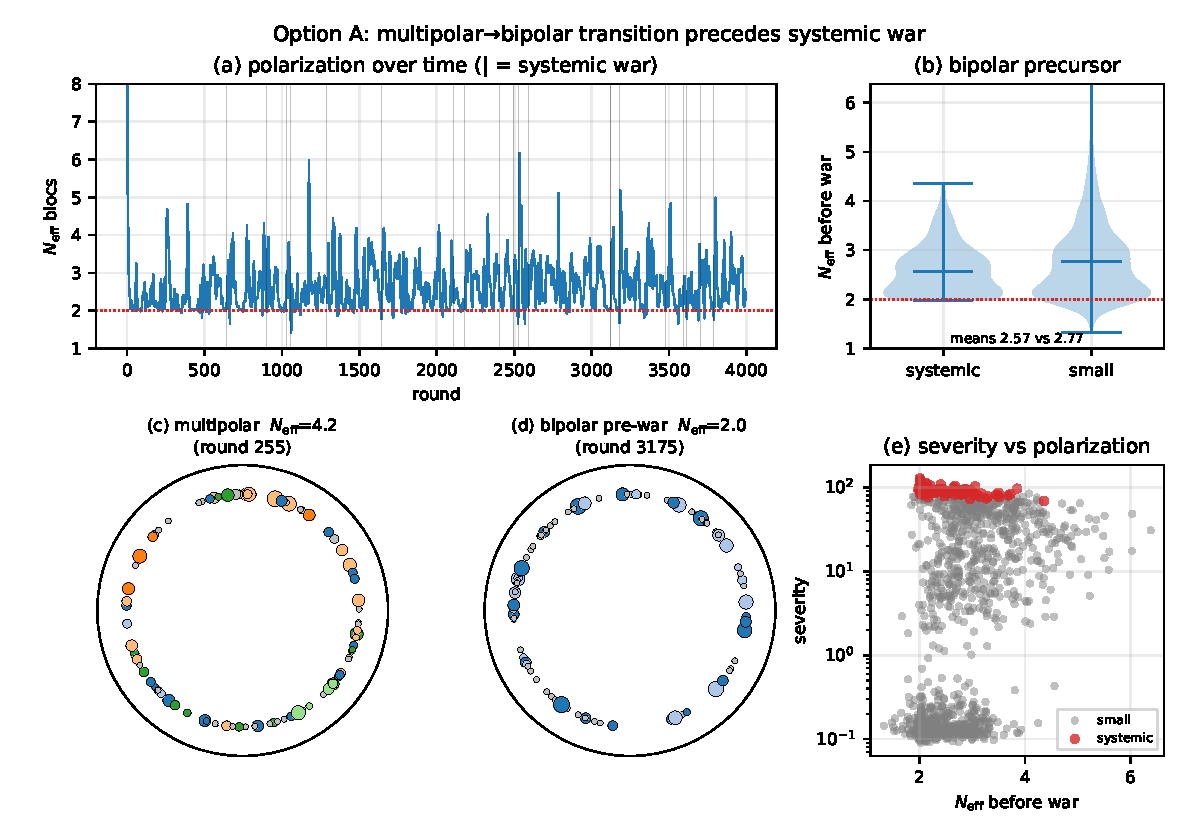
\includegraphics[width=\textwidth]{figs/selforg_v2_optionA.pdf}
\caption{\textbf{Option A.} (a) $\Neff(t)$, 20 most severe wars marked; (b)
pre-war $\Neff$, systemic vs small; (c) a multipolar phase and (d) a bipolar
pre-war moment on the ring (dot size $\propto$ strength, colour $=$ alliance);
(e) severity vs pre-war $\Neff$.}
\label{fig:A}
\end{figure}

\paragraph{Option B --- with absorption, collective foresight is
destabilising.} Sweeping a frozen, homogeneous deliberation depth
$n\in\{1,\dots,64\}$ (3 seeds, 2500 rounds; Spearman $\rho$ vs $n$):
\begin{itemize}\itemsep1pt
\item \textbf{Systemic-war rate} rises from $13$ to $44$ per $1000$ rounds
  ($\rho=+0.96$).
\item \textbf{Length of peace} $\tau$ falls from $66$ to $22$ rounds
  ($\rho=-0.96$).
\item \textbf{Mean war severity} rises from $20$ to $30$ ($\rho=+0.93$).
\end{itemize}
This \emph{inverts} the result of the absorption-free variant (where foresight
kept the system multipolar and shrank wars). The reason is the new mechanism:
when winning a war means \emph{absorbing} your rival, a deeper-thinking state is a
better predator --- it more reliably identifies winnable conquests and the
pivotal moments to join, and exploits them. Collective foresight therefore
accelerates conquest and systemic war rather than deterring it.
\begin{quote}\itshape
With real conquest stakes, predictability is destabilising: the better states
foresee the outcome of war, the more often the winnable war is fought, and the
shorter the peace.
\end{quote}
(Here polarization $\Neff$ barely moves with $n$, $2.9\!\to\!3.1$; the lever is
opportunism, not bloc structure.)

\begin{figure}[h]
\centering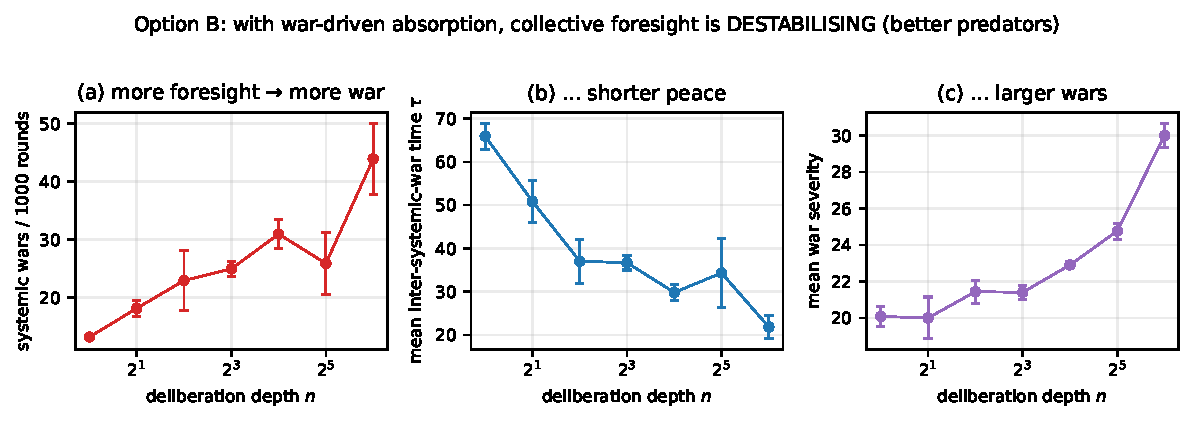
\includegraphics[width=\textwidth]{figs/selforg_v2_optionB.pdf}
\caption{\textbf{Option B.} Deliberation depth $n$ (log axis) as a control
parameter; mean $\pm$ sd over seeds.}
\label{fig:B}
\end{figure}

% ====================================================================
\section{Outlook}

The model now has the ingredients in the right places: endogenous rise-and-fall
of powers (dynamic $\gamma$), prediction as simulation (rollouts), balancing
alliances on a geography, and wars that reshape the alliance graph by absorption.
Natural next steps: (i) a 2-bloc mean-field / first-passage theory for the
inter-war time and the $\Neff$ precursor; (ii) test whether war severity is a
single function of $\Neff^{\rm pre}$ (one-parameter law); (iii) strengthen the
fitness coupling so deliberation depth self-organises to its cost-optimal value;
(iv) confront NMC/COW data --- is the major-power system near $\Neff\!\approx\!2$
before 1914/1939, and is relative-capability \emph{slope} the better war predictor?

\end{document}
